\documentclass{article}
\usepackage[utf8]{inputenc}
\usepackage{tikz}
\usetikzlibrary{shapes.geometric, arrows}
\renewcommand\familydefault{\sfdefault}

\tikzstyle{startstop} = [rectangle, rounded corners, text width=3cm, minimum width=3cm, minimum height=1cm,text centered, draw=black, fill=red!50]

\tikzstyle{io} = [trapezium, trapezium left angle=70, trapezium right angle=110, text width=3cm, minimum width=3cm, minimum height=1cm, text centered, draw=black, fill=blue!50]

\tikzstyle{process} = [rectangle, text width=3cm, minimum width=3cm, minimum height=1cm, text centered, draw=black, fill=orange!70]

\tikzstyle{decision} = [diamond, text width=3cm, minimum width=3cm, minimum height=1cm, text centered, draw=black, fill=green!50]

\tikzstyle{arrow} = [thick,->,>=stealth]

\begin{document}
\pagenumbering{gobble}
\section*{\centering{Houdini Message Receiver}}

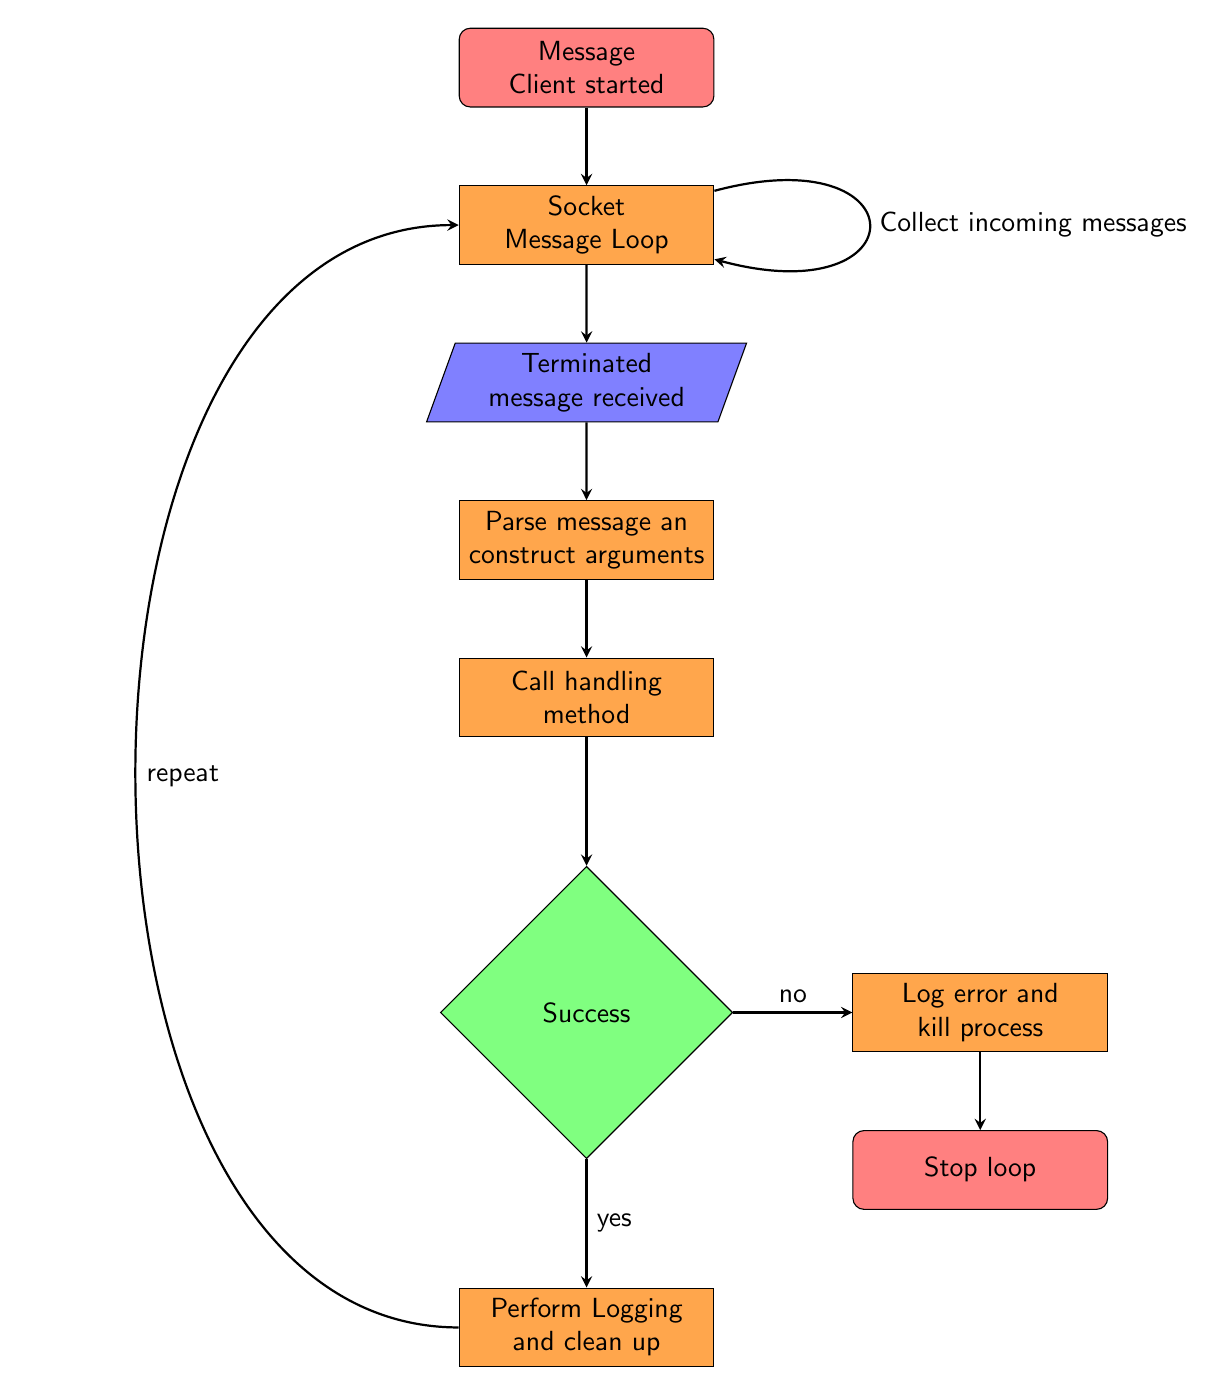
\begin{tikzpicture}[node distance=2cm]

\node (start) [startstop] {Message Client started};
\node (ioLoop) [process, below of=start] {Socket \mbox{Message} Loop};
\node (msgReceived) [io, below of=ioLoop] {Terminated message received};
\node (parse) [process, below of=msgReceived] {Parse message an construct arguments};
\node (call) [process, below of=parse] {Call \mbox{handling} method};
\node (success) [decision, yshift=-2cm, below of=call] {Success};
\node (done) [process, yshift=-2cm, below of=success] {Perform Logging and clean up};
\node (fail) [process, xshift=3cm, right of=success] {Log error and kill process};
\node (stop) [startstop, below of=fail] {Stop loop};

\draw [arrow] (start) -- (ioLoop);
\draw [arrow, loop right] (ioLoop) to node [anchor=west] {Collect incoming messages} (ioLoop);
\draw [arrow] (ioLoop) -- (msgReceived);
\draw [arrow] (msgReceived) -- (parse);
\draw [arrow] (parse) -- (call);
\draw [arrow] (call) -- (success);
\draw [arrow] (success) -- node [anchor=west] {yes} (done);
\draw [arrow] (success) -- node [anchor=south] {no} (fail);
\draw [arrow] (fail) -- (stop);
\draw [arrow, out=180, in=180] (done) to node [anchor=west] {repeat} (ioLoop);

\end{tikzpicture}

\end{document}